\documentclass[mathpazo]{aamm}
%%%%% journal  info %%%%%%%%%
\setcounter{page}{1}
\renewcommand\thisnumber{x}
\renewcommand\thisyear {2016}
\renewcommand\thismonth{xxx}
\renewcommand\thisvolume{xx}
%%%%%%%%   end  %%%%%%%%%%%%%

%%%%% author macros %%%%%%%%%
% place your own macros HERE
\usepackage{algorithmic} 
\usepackage[]{algorithm}
\newcommand{\bmx}{x}
\newcommand{\Real}{\mathbb{R}}
\newcommand{\eps}{\varepsilon}
%%%%% end %%%%%%%%%

\begin{document}

%%%%% title and author(s):
% \markboth{Author(s)}{Short Title}
% \title{Title}

\markboth{Y. Huang and K. Jiang}{Stick Hill-Climbing Algorithm}
\title[Hill-Climbing Algorithm with a Stick] {
Hill-climbing algorithm with a stick for unconstrained optimization problems}

%same address:
\author[Y. Huang and K. Jiang]{Yunqing Huang\corrauth and Kai Jiang}
%\address{address of AUTHOR1, AUTHOR2 and AUTHOR3}
\address{
Hunan Key Laboratory for Computation and Simulation in Science and Engineering, 
\\
Key Laboratory of Intelligent Computing \& Information Processing of Ministry of Education, 
\\ School of Mathematics and Computational Science,
Xiangtan University, Xiangtan {\rm 411105}, China }

\emails{{\tt huangyq@xtu.edu.cn} (Y. Huang), {\tt
kaijiang@xtu.edu.cn} (K. Jiang)}


%%%%% Begin Abstract %%%%%%%%%%%
\begin{abstract}
Inspired by the behavior of the blind for hill-climbing using a
stick to detect a higher place in the form of circle, 
we propose a heuristic direct search method to
solve the unconstrained optimization problems. 
Instead of searching a neighbourhood of the current point as done
in the traditional hill-climbing, or along specified search
directions in standard direct search methods, the new algorithm
searches on a surface with radius determined by the motion of the stick.
The significant feature of the proposed algorithm is that it only has one
parameter, the search radius, which makes the
algorithm convenient in practical implementation.
The developed method can shrink the search space to a closed ball, or
seek for the final optimal point by adjusting search radius. 
Furthermore our algorithm possesses multi-resolution
feature to distinguish the local and global optimum points  
with different search radii.
Therefore, it can be used by itself or integrated with other
optimization methods flexibly as a mathematical optimization technique.
A series of numerical tests, including high-dimensional problems,
have been well designed to demonstrate its performance.
\end{abstract}
%%%%% end %%%%%%%%%%%

%%%%% Keywords %%%%%%%%%%%
\keywords{direct search algorithm, stick hill-climbing
algorithm, search radius} 

%%%% AMS subject classifications %%%%
 \ams{90C56, 90C30, 56K05}

%%%% maketitle %%%%%
\maketitle

%%%% Start %%%%%%
\section{Introduction}
\label{sec:intro}

For simplicity, we limit our discussion to the following
unconstrained optimization problem
\begin{align*}
	\max_{\bmx\in\Omega}f(\bmx),~~~ \Omega\subset\Real^n,
\end{align*}
where $f:\Real^n\to\Real$.
The following statements are also suitable to find the minima of
objective function with constraint conditions.
There have been innumerable approaches developed to solve these
optimization problems. These methods usually can be divided into
two types, derivative-based methods and derivative-free methods,
depending on whether they use derivative information or not. 
The derivative-based approaches appeal to the Taylor's series
expansion of the objective function\,\cite{sun2006optimization,
conn2000trust,nocedal2006numerical}. For example, the
steepest descent method assumes the availability of first
derivatives and uses the first-order Taylor polynomial to
construct local linear approximations of $f$. 
Newton's method assumes the availability of first
and second derivatives and uses the second-order Taylor
polynomial to construct local quadratic approximations of $f$.
However, for a variety of reasons there have always been many
instances where (at least some) derivatives are unavailable or
unreliable, or finite-difference derivative approximation is
unavailable or available at a prohibitive cost. 
Some of the reasons contain increasing complexity in
mathematical modeling, higher sophistication of scientific
computing, an abundance of legacy codes, and data
science\,\cite{conn2009introduction}. Nevertheless, under such
circumstances it may still be desirable to carry out
optimization. It follows that the derivative-free optimization
technique is required. 

The derivative-free optimization is an area of long history and
current rapid growth in the scientific and engineering communities. 
The derivative-free algorithms can mainly be classified as direct and
model-based\,\cite{rios2013derivative}.
Direct algorithms usually determine search directions by evaluating the
function $f$ directly, whereas model-based algorithms construct
and utilize a surrogate model of $f$ to guide the search process.
Recently developed methods based trust-region using
interpolation model are in this category\,\cite{powell2000uobyqa,
powell2002trust, wu2009heuristic, zhang2014sobolev}. 
In practical implementation, heuristic algorithms, such as
simulated annealing, genetic algorithm, neural networks, and deep
learning\,\cite{michalewicz2004how, lecun2015deep}, have been also
developed to solve derivative-free optimization.
Here we focus our attention on the direct search algorithms.

The term ``direct search'', firstly coined by Hooke and
Jeeves in 1961 year\,\cite{hooke1961direct}, is used to describe 
a sequential examination of trial generated by a
certain strategy. From a modern viewpoint, the direct search
methods neither compute nor approximate
derivatives\,\cite{lewis2000direct}. 
A popular direct search method is the
Nelder-Mead simplex algorithm\,\cite{nelder1965simplex}. The
algorithm starts with a set of points that form a simplex.
In each iteration, the objective function values at the corner
points of the simplex determine the worst corner point. The
algorithm attempts to replace the worst point by introducing a
new vertex by a reflection, an expansion, or a contraction
operator that results in a new simplex. 
Another class of direct search methods are the directional
direct-search methods, including the
original Hooke-Jeeves algorithm\,\cite{hooke1961direct}, the
coordinate-, or compass-search methods, pattern-search
methods\,\cite{conn2009introduction}, generalized 
pattern search method\,\cite{torczon1997convergence}, and 
generating set search method\,\cite{kolda2003optimization}.
A multidirectional search algorithm, regarded as both a directional and a simplicial
direct search method, has been also proposed by 
Dennis and Torczon\,\cite{dennis1991direct}.
The common ground of these directional direct-search methods is
that they incorporate some mechanism to choose ascend directions
and search along these directions with an appropriate step length
from the current iterate for a new iterate with a higher function value.
The same is done by derivative-based algorithms to
enforce global convergence\,\cite{sun2006optimization, nocedal2006numerical}.
However the predetermined search direction set 
may contain none of ascend or descent direction.
Moreover, due to the absence of derivative information, the
search directions could not be adjusted flexibly according to
$f$\,\cite{conn2009introduction}. 
Under such circumstances, the directional direct search methods
fail to converge on this function.
Recently, Gratton et al.\,\cite{gratton2015direct}
analyzed the convergent properties of direct-search algorithms
when the search direction are probabilistic descent. 

Our method is inspired by the behavior of the blind for
hill-climbing that they find a high position with help of a stick using
circular motions, usually without a priori information. 
Based on the observation, we propose a new search strategy
that the search set is a closed manifold in each iteration, for
example, a circle in two dimensions, a spherical surface in
higher dimensions, rather than a neighbourhood of current iterate as done in
traditional hill-climbing methods\,\cite{russell2010artificial}.
An example of the search set in two dimensions is presented in Fig.\,\ref{fig:idea},
\begin{figure}[!htbp]
	\centering
	  \includegraphics[scale=0.35]{./nc.png}
	\caption{The schematic image demonstrates how to choose the search set
	from the traditional hill-climbing method to our proposed
	algorithm in two dimensions. In the traditional hill-climbing
	method, the search set is a neighbourhood of current iterate,
	while in our method, that is a closed surface, here a compass.}
\label{fig:idea}
\end{figure}
Then we compare function values on the closed
manifold with the current iterate. 
It follows that the iterate is replaced once a higher function
value on the manifold has been found.
The new formed optimization method dose not predetermine the search
directions. More importantly, it has a unique parameter, the 
radius of the circle or the spherical surface, which makes the
algorithm convenient in practical implementation.

%The hill-climbing search algorithm is one of the most basic locally
%direct search technique. In original hill-climbing, at each step the current
%node is replaced by a better neighbourhood with the higher function
%value.  It terminates when it reaches a ``peak'' where no
%neighbourhood has a higher value. The algorithm does not maintain a
%search history, so the data structure for the current node need
%only record the state and the value of the objective function.
%The hill-climbing often makes rapid progress toward a solution
%because it is usually quite easy to improve a bad state. 
%The relative simplicity of the algorithm makes it popular in
%computer science, such as artificial
%intelligent\,\cite{russell2010artificial}.
%Unfortunately, hill-climbing often gets stuck when the objective
%function has the following landscape: local maxima, ridges, or plateaux. 
%A series of variants have been also developed to improve the simple
%version, including steepest ascent hill-climbing, stochastic
%hill-climbing, and random-restart
%hill-climbing algorithms\,\cite{russell2010artificial}.  

%Inspired by the behavior of the blind with a stick for
%hill-climbing, in this paper, we propose a new class of direct
%search methods to solve unconstrained optimization problems. 
%The basic idea of the new algorithm, at each iteration, 
%is comparing function values on a closed surface, such as a
%compass in two dimensions, and a spherical surface in high
%dimensions, of the current node with radius determined by the
%stick, rather than the neighbourhoods of current node. 
%It follows that the centre node is replaced by another point on
%the closed surface if it has higher function value. 
%The significant feature is the proposed approach has 
%a unique parameter, the search radius, which makes the
%algorithm convenient in practical implementation.
%\begin{figure}[!htbp]
%    \centering
%      \includegraphics[scale=0.35]{./nc.png}
%    \caption{The schema demonstrates how to choose the search set
%    from the traditional hill-climbing method to our proposed
%    algorithm in two dimensions. In the traditional hill-climbing
%    method, the search set is a neighbourhood of current iterate,
%    while in our method, that is a closed surface, here a compass.}
%\label{fig:idea}
%\end{figure}
%Fig.\,\ref{fig:idea} shows the basic idea of our proposed
%algorithm of choosing the search set, compared with the
%traditional hill-climbing method, in two dimensions.

In the following, we will give a concrete and
feasible numerical algorithm in Sec.\,\ref{sec:algorithm}. 
The length of the radius is determined by the motion of the
stick, therefore, it can be adjusted during the iteration procedure.
Correspondingly, a regulated search radius method is also
presented in this section.
In contrast to the above-mentioned directional direct search
algorithms, our algorithm does not incorporate the search directions. 
A large number of numerical tests are showcased in
Sec.\,\ref{sec:experiment}. Numerical results demonstrate that
the new algorithm has finite-step convergence, and is able to
distinguish the local and global optimum points with different
search radii. Finally the conclusion and discussions are given
in Sec.\,\ref{sec:conclusion}.

\section{Algorithm description}
\label{sec:algorithm}

For convenience, we introduce some notations before the algorithm
description. $f(\bmx)$ is the objective function. $\bmx^*$ is one
of the maximizers of $f(\bmx)$ which may be local or global.
$\bmx_0$ is the initial position when starting the optimization method, and
$\bmx_k$ is the $k$-th iterate.
$\rho$ is the search radius determined by the stick. $O(\bmx_k, \rho)=\{\bmx:
|\bmx-\bmx_k|=\rho\}$ is the search surface in the
$k$-th iteration with radius $\rho$. $\Omega(\bmx_k,
\rho)$ is the neighbourhood of $\bmx_k$ with radius of $\rho$.
In what follows, we will propose the heuristic algorithm and point out
that it can capture the area of maximizers. 

\begin{algorithm}[]
	\caption{Stick Hill-Climbing Algorithm} 
	\label{alg:CHC}
\begin{algorithmic}[]
	\STATE \textbf{Initialization:} Choose $\bmx_0$ and $\rho$.
	\STATE \textbf{For} $k=0,1,2,\dots$
	\STATE \hspace{0.5cm} Try to find $\bar{\bmx}\in O(\bmx_k,
	\rho)$
		   such that $f(\bar\bmx)>f(\bmx_k)$. 
			\\
		 \hspace{0.5cm} If such a point is found, then set $\bmx_{k+1}= \bar\bmx$.
		  \\
	 	  \hspace{0.5cm} Otherwise, terminate the iteration.
\end{algorithmic}
\end{algorithm}
Algorithm\,\ref{alg:CHC} is the proposed method, the hill-climbing algorithm with a stick.
For simplicity, we name it stick hill-climbing algorithm. 
For each $k$ step, there are three possible circumstances in 
Algorithm\,\ref{alg:CHC} to determine whether to stop the iteration or not. 
The first case is $f(\bmx)<f(\bmx_k)$, for all $\bmx\in O(\bmx_k,
\rho)$. The iteration is terminated, and the algorithm can declare
that there is at least one maximizer in the neighbourhood of $\Omega(\bmx_k,
\rho)$ if the objective function $f$ satisfies some conditions, such as continuity.
The second situation is $f(\bmx)\leq f(\bmx_k)$, i.e., there exists 
$\bar\bmx\in O(\bmx_k, \rho)$ such as $f(\bar\bmx)=f(\bmx_k)$.
We let $\bmx_{k+1}= \bar\bmx$, and continue the iteration.
The third case is $f(\bmx)\equiv f(\bmx_k)$ for all
$\bmx\in O(\bmx_k, \rho)$. Then the method of current 
version can not infer the existence of maximizers or minimizers
in $\Omega(\bmx_k, \rho)$. However we can increase or
decrease the search radius $\rho$ as the below Algorithm\,\ref{alg:pCHC}
suggested, and further run Algorithm\,\ref{alg:CHC} to find the
location of maximizers. 

The search set of the developed algorithm is the surface
$O(x_k, \rho)$ of the current iterate $x_k$ with radius
$\rho$, rather than the
neighbourhoods of $x_k$ as done in the traditional hill-climbing.
The developed algorithm tries to search for the neighbourhood of
maximizers rather than to find the maximizer directly.
Moreover, the distance between the extreme points and the
convergent iterate is not more than $\rho$.
If $\rho$ is driven to zero, the monotonic increasing sequence
$ \{f(\bmx_k)\}$ produced by the stick hill-climbing algorithm
implies $\{\bmx_k\}$ approximates a maximizer.
Therefore, the search radius $\rho$ is a natural choice to
represent the approximate error of the stick hill-climbing algorithm. 

In practice, we have to sample the observed
points set in each iteration for Algorithm\,\ref{alg:CHC}.
Obviously, there exist lots of ways to accomplish it, such as
randomly, adaptively, or uniformly sampling. Here we
choose a dynamic refinement principle to sample the search surface 
in each iteration rather than a dense mesh from the start, as
Algorithm\,\ref{alg:refined} shows.
\begin{algorithm}[]
	\caption{Dynamic Refinement Technique} 
	\label{alg:refined}
\begin{algorithmic}[]
	\STATE For $k$ iteration in Algorithm\,\ref{alg:CHC}
	\STATE ~~\textbf{Step 1}. Sample the surface
	$O(\bmx_k, \rho_k)$ with a coarse mesh. \\
	\STATE ~~\textbf{Step 2}. Compare the function values of the
	samples with $f(\bmx_k)$.
	\\
	\hspace{1.5cm} If there exists $\bar\bmx$ such that
	$f(\bar\bmx)>f(\bmx_k)$, goto \textbf{Step 4}.
	\\
	\hspace{1.5cm} Otherwise, goto \textbf{Step 3}.
	\STATE ~~\textbf{Step 3}. Subdivide $O(\bmx_k, \rho_k)$, goto
	\textbf{Step 2}.
	\STATE ~~\textbf{Step 4}. Declare that the iteration is
	successful, and set $\bmx_{k+1}= \bar\bmx$.
\end{algorithmic}
\end{algorithm}
For $k$ iteration in Algorithm\,\ref{alg:CHC}, we firstly use
a coarse mesh to sample $O(\bmx_k, \rho_k)$. By comparing the
function values of these samples with $f(\bmx_k)$,
Algorithm\,\ref{alg:refined} determines whether the current grid
shall be refined or not. The technique can reduce the number of
the function evaluations.
\begin{figure}[!htbp]
	\centering
	  \includegraphics[scale=0.45]{./sketch.png}
	\caption{Schematic diagram of equally refined approach for
	sampling the search surface $O(\bmx_k, \rho)$ in two
	dimensions, i.e, a circle. Subfigure (a) demonstrates the initial samples,
	and images (b-d) show new sample points in the equally
	refined process sequentially.}
\label{fig:obset:sketch}
\end{figure}
For example, in two dimensions, the search set is a circle.
The schematic plot of the equally
refined method is presented in Fig.\,\ref{fig:obset:sketch} when
the maximum sample points $N_{\rm{max}}=32$.
For $n$-dimensional ($n\geq 3$) optimization problems, the search
areas are restricted to an $n$-dimensional spherical surface.
In these cases, we use the generalize spherical coordinate
transformation to obtain the position of samples, i.e.,
\begin{align*}
	x^1_{k+1} &= x^1_{k}+\rho_{k}\cos(\phi^1),
	\\
	x^2_{k+1} &= x^2_{k}+\rho_{k}\sin(\phi^1)\cos(\phi^2),
	\\
	& \dots
	\\
	x^{n-1}_{k+1} &= x^{n-1}_{k}+
	\rho_{k}\sin(\phi^1)\cdots\sin(\phi^{n-2)}\cos(\phi^{n-1}),
	\\
	x^{n}_{k+1} &=
	x^{n}_{k}+\rho_{k}\sin(\phi^1)\cdots\sin(\phi^{n-2)}\sin(\phi^{n-1}),
\end{align*}
where $\phi^1,\cdots\phi^{n-2}\in[0,\pi]$, $\phi^{n-1}\in[0,2\pi)$.
Then one can discrete the angular coordinates,
$\phi^1,\cdots\phi^{n-1}$, by the equally refined method in a
dynamical way.  In practice, we discretize $\phi^1, \phi^2,
\cdots, \phi^{n-1}$ using $[m,m,\cdots,2m]$ points at start,
and let $m\leftarrow m+k$ ($k\in \mathbb{Z}^+$) in the
refinement process. The process is terminated when $2m^{n-1}$ is
greater than a given $N_{max}$.  

If the stick hill-climbing algorithm converges, it is evident that
the search space is shrunk to a ball with the radius $\rho$. 
The convergent point $\bmx_k$ provides a good initial value for
other optimization methods, including derivative-free
approaches, and derivative-based algorithms if the objective
function is differentiable. 
We will demonstrate this by several numerical experiments in
Sec.\,\ref{sec:experiment}.
Meanwhile, we can further exploit the potential of
stick hill-climbing algorithm to improve the precision by tuning the
search radius $\rho$. Algorithm\,\ref{alg:pCHC} presents a
strategy to resize the search radius $\rho$. 
Significant difference of the version from
Algorithm\,\ref{alg:CHC} is adjusting the search radius
$\rho$ when Algorithm\,\ref{alg:CHC} fails to find
$f(\bar\bmx)>f(\bmx_k)$, $\bar{\bmx}\in O(\bmx_k, \rho)$ with
fixed $\rho$. 
The natural stop criterion of Algorithm\,\ref{alg:pCHC} is to
terminate the run when $\rho$ is smaller than a prescribed
numerical accuracy.
Certainly, the search surface can be expanded by setting
control factor $\eta>1$ if required. 
In fact, Algorithm\,\ref{alg:pCHC} provides a restart technique by
fixed the $k$-iterate with different search radius $\rho$.

\begin{algorithm}[]
	\caption{Changeable Stick Hill-Climbing Algorithm} 
	\label{alg:pCHC}
\begin{algorithmic}[]
	\STATE \textbf{Initialization:} Choose $\bmx_0$, $\rho$,
	and control factor $\eta$.
	\STATE \textbf{For} $k=0,1,2,\dots$
	\STATE \hspace{0.5cm} Use Algorithm\,\ref{alg:CHC} to find
	$\bar{\bmx}\in O(\bmx_k, \rho)$ such that
	$f(\bar\bmx)>f(\bmx_k)$.
		 \\
		 \hspace{0.5cm} If such a point is found, then set
						 $\bmx_{k+1}= \bar\bmx$.
		  \\
	 	  \hspace{0.5cm} Otherwise, change the search radius
		  $\rho = \eta \cdot \rho$.
\end{algorithmic}
\end{algorithm}

\section{Numerical results}
\label{sec:experiment}

In this section, we choose three kinds of test functions,
including single extreme point function, multi-extreme points
function, and continuous but indifferentiable function, 
to demonstrate the performance of the stick hill-climbing algorithm. 
The maximum number of sampling points $N_{\rm{max}}$ for search
set in Algorithm\,\ref{alg:refined} defaults to $16$ if not
specified (see Fig.\,\ref{fig:obset:sketch}\,(a)-(c)).

\subsection{Single extreme point function}
\label{subsec:max1}

For the first example we consider two-dimensional Gaussian function
\begin{align}
	f(x,y) = h\exp\left(-\frac{x^2}{s_x}-\frac{y^2}{s_y}\right),
	\label{eqn:exp1}
\end{align}
where $h=10$, $s_x =1.0$, $s_y = 0.5$.
The graph of a Gaussian function likes a ``bell'' sharp, and has
a unique maximum, $(x^*, y^*)=(0,0)$, and $f(0,0)=10$.
The objective function is differentiable in $\Real^2$, however,
it quickly falls off towards zero out of the ``bell''. 

We firstly investigate the influence of initial values for the
stick hill-climbing algorithm. For this set of tests of 20 runs, 
the search radius $\rho$ is fixed as $1.0$, start points are
randomly generated in the space $(-10, 10)^2$. For each
experiment, the stick hill-climbing method can capture a neighbourhood of the peak
$(0,0)$ in finite iterations. Fig.\,\ref{fig:exp1:randInit} gives
the required iterations for convergence in $20$ numerical experiments.
\begin{figure}[!htbp]
	\centering
	\includegraphics[scale=0.3]{./gaussrandInit.png}
	  \caption{The iterations of convergence of the stick
	  hill-climbing algorithm to the single-peak Gaussian function
	  \eqref{eqn:exp1} in 20 runs.  Start points are randomly
	  generated in the space $(-10, 10)^2$, and $\rho=1.0$. 
	  The flat dashed line shows the average.} 
	  \label{fig:exp1:randInit}
\end{figure}
In these $20$ runs, the average iterations of convergence is
about $12$, while the maximum is $20$, and the minimum is $5$.
The number of iterations is inversely proportional to the
distance of the initial point and the optimal point.
When the initial values are far away from the optimal point, the
algorithm needs more iterations. In contrast, when the initial
points are close to the maximizer, the method requires less iterations. 
We also note that when the start point is far away from the peak,
the derivative-based methods, such as steepest descent method,
conjugate gradient method and Newton method, will fail since the
gradient value is almost zero. 
However, the stick hill-climbing algorithm can always approximate the
peak point. The initial values may yield a few more iterations
but NOT affect the convergence.

Then we take an example to further observe the numerical behavior
of the stick hill-climbing algorithm.
Tab.\,\ref{tab:gauss:CHC} shows the iterative procedure of the
stick hill-climbing approach in detail when the start point is
$(x_0, y_0)=(3.3, 2.9)$ with fixed search radius $\rho=1.0$. 
\begin{table}[!htbp]
\caption{\label{tab:gauss:CHC}The iterative procedure of stick
hill-climbing algorithm with $\rho=1.0$ when the initial value
is $(x_0, y_0)=(3.3, 2.9)$.}	
\begin{center}
	\footnotesize{
\begin{tabular}{|c|c|c|c|}
 \hline
 $k$ & $(x_k,y_k)$ & $f(x_k,y_k)$ & $|f(x_k,y_k)-f(x^*,y^*)|$
 \\ \hline
 0 & (3.3, 2.9) & $9.24059\times 10^{-12}$ & 9.999999999990759
 \\ \hline
 1 & (3.3, 1.9) & $1.36435\times 10^{-7}$ & 9.999999863564643  
 \\\hline
 2 & (2.3, 1.9) & $3.68957\times 10^{-5}$ & 9.999963104276466
 \\\hline
 3 & (2.3, 0.9) &  $9.97758\times 10^{-3}$ &  9.990022422035157
 \\\hline
 4 & (1.3, 0.9) & 0.36516 &  9.634838262462596
 \\\hline
 5 & (0.3, 0.9) & 1.80866    &  8.191342073828778
 \\\hline
 6 & (0.3, -0.1) & 8.95834   &  1.041658647034717
 \\\hline
\end{tabular}
}
\end{center}
\end{table}
The results show that the iterates can be updated efficiently to
capture the neighbourhood of the maximizer $(0,0)$ within $6$ steps. 
The convergent result reduces the search space and
provides a good start position $(0.3, -0.1)$ to further
approximate the maximizer to high precision with other
optimization algorithms.

Due to the good analytical nature of objective function, the
derivative-based methods are good choices for finding the
maximizer with the above convergent results. For our purpose, we
still adopt the stick hill-climbing method, but with changeable $\rho$ to
approximate the peak (see Algorithm\,\ref{alg:pCHC}), and observe
its numerical behavior. 
\begin{table}[!htbp]
\caption{\label{tab:gauss:pCHC}The iterative procedure of the
changeable $\rho$ compass hill-climbing
algorithm\,\ref{alg:pCHC} with control factor $\eta=0.5$ when the
start point is $(x_0, y_0)=(0.3, -0.1)$, and initial search
radius $\rho=0.8$.  $k_\rho$ represents the number of
iterations for a given $\rho$.}		
\begin{center}
	\footnotesize{
\begin{tabular}{|c|c|c|c|c|}
 \hline
 $\rho$ & $k_{\rho}$ & $(x_k,y_k)$ & $f(x_k,y_k)$ & $|f(x_k,y_k)-f(x^*,y^*)|$
 \\ \hline
 0.8 & 1 & (0.3, -0.1) &  8.9583413  &  1.04166
 \\ \hline
 0.4 & 2 & (-0.1, -0.1) & 9.7044553   &  $2.95545\times 10^{-2}$
 \\ \hline
 0.2 & 2 & ($4.14214\times 10^{-2}, 4.14214\times 10^{-2}$) & 9.9486604  & $5.13396\times 10^{-2}$
 \\ \hline
 0.1 & 2 & ($-2.92893\times 10^{-2}, -2.92893\times 10^{-2}$) & 9.9742972 & $2.57028\times 10^{-2}$ 
 \\ \hline
 $5\times 10^{-2}$ & 4 & ($-1.46447\times 10^{-2}, -1.46447\times 10^{-2})$ & 9.9935681& $6.43191\times 10^{-3}$ 
 \\ \hline
 $2.5\times 10^{-2}$ & 4 & ($-7.32233\times 10^{-3},-7.32233\times 10^{-3}$) & 9.9983916   & $1.60837\times 10^{-3}$
 \\ \hline
 $1.25\times 10^{-2}$ & 4 & ($-3.66117\times 10^{-3}, -3.66117\times 10^{-3}$) & 9.9995979  &  $4.02116\times 10^{-4}$
 \\ \hline
 $6.25\times 10^{-3}$ & 4 & ($7.58252\times 10^{-4}, 7.58252\times 10^{-4}$) & 9.9999272   & $7.27699\times 10^{-5}$ 
 \\ \hline
 $3.125\times 10^{-3}$ & 4 & ($-9.15291\times 10^{-4},-9.15291\times 10^{-4}$) & 9.9999749 & $2.51327\times 10^{-5} $
 \\ \hline
 $1.5625\times 10^{-3}$ & 2 & ($1.895630\times 10^{-4},1.895630\times 10^{-4}$) & 9.9999989 & $1.07802\times 10^{-6}$
 \\ \hline
\end{tabular}
}
\end{center}
\end{table}
The start node is $(0.3, -0.1)$, the initial search radius is
$\rho_0=0.8$. 
The control factor $\eta$ in Algorithm\,\ref{alg:pCHC} is set to
be $0.5$ under which circumstances the search radius can be
driven to decrease during iteration. Tab.\,\ref{tab:gauss:pCHC}
shows that, in $29$ ($\sum k_\rho$) steps,
Algorithm\,\ref{alg:pCHC} can efficiently obtain a neighbourhood
of the maximizer $(0,0)$, while the error of $|f(x_{29},
y_{29})-f(0,0)|$ achieves about $O(10^{-6})$.

\subsection{Multi-extreme points function}
\label{subsec:minmulit}

The second tested function is the Ackley
function\,\cite{dieterich2012empirical},
a benchmark function, widely used for
testing optimization algorithms.
The expression of the Ackley function can be written as
\begin{align}
	f(\bmx) =
	-a\cdot\exp\left(-b\cdot\sqrt{\frac{1}{n}\sum_{i=1}^2
	x_i^2}\right)-
	\exp\left(\frac{1}{n}\cos(c x_i)\right)+a+\exp(1),
	\label{eqn:ackley}
\end{align}
where $a=20, b=0.2, c=2\pi$, $n$ is the dimension.
Ackley function has many local minima and a unique global
minimum of $(0,0)$ with $f(0,0)=0$, which poses a risk for
optimization algorithms to be trapped into one of local
minima, such as the traditional hill-climbing method\,\cite{back1996evolutionary}.
\begin{figure}[!htbp]
	\centering
	  \includegraphics[scale=0.35]{./ackley.png}
	  \caption{Morphology of 2-dimensional Ackley function \eqref{eqn:ackley}.}
\label{fig:ackley}
\end{figure}
In this subsection, we will apply the stick hill-climbing
algorithm to 2-, 4-, 6-, 8-dimensional Ackley function. 

Firstly we consider the 2-dimensional Ackley function whose   
morphology is shown in Fig.\,\ref{fig:ackley}.
\begin{figure}[!htbp]
	\centering
	\includegraphics[scale=0.3]{./ackleyrandInit.png}
	  \caption{The required iterations of convergence by stick hill-climbing
	  algorithm\,\ref{alg:CHC} for Ackley function
	  \eqref{eqn:ackley} in 20 numerical experiments. 
	  Start points are randomly generated in the space
	  $(-12, 12)^2$ with fixed $\rho=1.0$.
	  The flat dashed line shows the average.} 
	  \label{fig:ackley:randInit}
\end{figure}
We want to examine the ability of Algorithm\,\ref{alg:CHC} to
approximate the global minimum. The first numerical
examples are also set to observe the influence of initial values
with fixed $\rho$. 
When $\rho=1.0$, $20$ numerical tests are performed with
random initial points generated in the space of $(-12, 12)^2$.
The convergent domain in each test contains the global minimizer $(0,0)$.
Fig.\,\ref{fig:ackley:randInit} shows the required iterations
for convergence. In the $20$ numerical tests, the average iterations of
convergence is about $15$, while the maximum number of
iterations is $23$ and the minimum is $5$. 
The initial positions also only affect the
speed of convergence, but not the ability of catching the
neighbourhood of the global minimum.

\begin{table}[!htbp]
\caption{\label{tab:ackley:CHC}The iterative procedure of the stick
hill-climbing algorithm with fixed $\rho=1.0$ when the initial
value is $(x_0, y_0)=(4.1, 3.4)$. For Ackley function, the global
minimum is $(x^*, y^*)=(0,0)$, and $f(x^*,y^*)=0$.}
\begin{center}
	\footnotesize{
\begin{tabular}{|c|c|c|}
 \hline
 $k$ & $(x_k,y_k)$ & $|f(x_k,y_k)-f(x^*,y^*)|$
 \\ \hline
0 & (4.1, 3.4) & 12.301695
 \\ \hline
1 & (3.1, 3.4) & 11.284588
 \\ \hline
2 & (3.1, 2.4) & 10.230367
 \\ \hline
3 & (2.1, 2.4) &  8.978451
 \\ \hline
4 & (2.1, 1.4) &  7.721871
 \\ \hline
5 & (1.1, 1.4) & 6.170178
 \\ \hline
6 & (1.1, 0.4) & 4.769384
 \\ \hline
7 & (0.1, 0.4) & 2.851124 
 \\ \hline
8 & (1.02388, 0.01732) & 2.719632 
 \\ \hline
9 & (0.02388, 0.01732) & 0.106464
 \\ \hline
\end{tabular}
}
\end{center}
\end{table}
To make this point clear, Tab.\,\ref{tab:ackley:CHC} gives the
iterative procedure in detail when the start position is $(x_0,
y_0)=(4.1,3.4)$, and $\rho=1.0$. 
One can see that the stick hill-climbing algorithm has ability to
find a neighbourhood of the global minimum in $9$ iterations.
The convergent point $(x_9, y_9)$ is close to the global minimizer $(0,0)$. 
As the above subsection done, we can also resize the search radius
$\rho$ in the stick hill-climbing algorithm to further approximate the global minimum.
If the initial search radius is $\rho_0=1.0$, and control factor
$\eta=0.5$, the changeable stick hill-climbing scheme costs $47$ iterations to reach an
error of $\rho_{\rm tol}=10^{-6}$. The convergent point is
$(3.170987\times 10^{-7}, 3.475996\times 10^{-7})$ which is much
closer to the global minimum $(0,0)$.

The above tests have demonstrated that the stick hill-climbing
algorithm can capture the neighbourhood of the global minimum of
the Ackley function. 
Subsequently we plan to manifest the ability of the stick
hill-climbing algorithm to obtain these local minimizers.
As discussed above, the unique regulatable parameter in the stick
hill-climbing scheme is the search radius $\rho$. Therefore we
will test the numerical behaviors with different size of $\rho$.
In the set of tests, the initial value is always $(x_0, y_0)=(4.1,3.4)$.
Tab.\,\ref{tab:ackley:r} gives the convergent results with
different $\rho$. Fig.\,\ref{fig:ackley:LG} marks
corresponding local minima.
\begin{table}[!htbp]
\caption{\label{tab:ackley:r}The convergent results and required
iterations of the stick hill-climbing algorithm with different
$\rho$ when the
initial value is $(x_0, y_0)=(4.1, 3.4)$. The locations of
different local minima are marked in Fig.\,\ref{fig:ackley:LG}.}
\begin{center}
	\footnotesize{
\begin{tabular}{|c|c|c|c|c|c|c|c|c|c|}
 \hline
 $\rho$ & 0.1 & 0.3 & 0.5 & 0.6 & 0.7 & 0.73 & 0.74 & 0.75 & 1.0
 \\\hline
 Iterations & 6   & 3   &  2  & 5   & 3   & 3    & 3    & 11   & 10
 \\\hline
 Minimizer & $\rm{Loc_1}$ & $\rm{Loc_1}$ & $\rm{Loc_1}$ &
 $\rm{Loc_4}$ & $\rm{Loc_2}$ & $\rm{Loc_2}$  &
 $\rm{Loc_3}$ & Global Min. & Global Min. 
 \\\hline
\end{tabular}
 }
\end{center}
\end{table}
\normalsize
\begin{figure}[!htbp]
	\centering
	  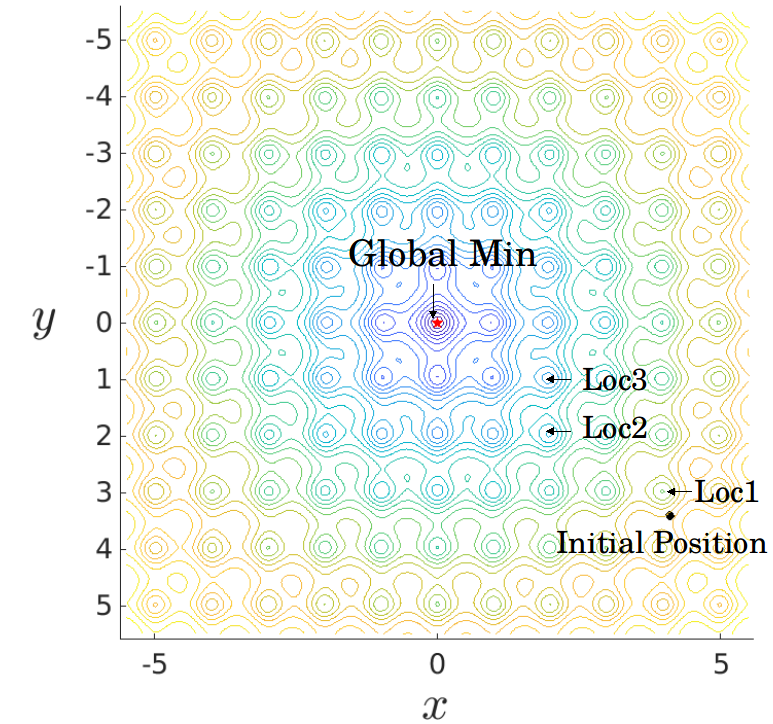
\includegraphics[scale=0.3]{./ackley_LG.png}
	  \caption{The locations of some local minima and the global
	  minimum of the Ackley function.}
\label{fig:ackley:LG}
\end{figure}
From these numerical experiments, one can find that the search
radius $\rho$ plays a filter role in
catching different local minimum by setting different values. 
When $\rho$ is greater than $0.75$, the stick hill-climbing
approach can approximate the global minimum, otherwise, the
method converges to the local minima. If starting from other
initial position, the stick hill-climbing can find other minima.

Next we consider the high-dimensional Ackley function, especially, 4-,
and 8-dimensional problems. In these numerical experiments, we
also choose the equally refine approach to sample the observed
spherical surface in a dynamic way in each iteration as mentioned
in Sec.\,\ref{sec:algorithm}.
The initial point $m=3$, and in each refinement procedure, we let
$m=m+1$. For 4-, and 8-dimensional problems, the maximum
samples $N_{max}$ is set as $800$ and $8000$,
respectively. The search radius $\rho$ is $1.0$ for 4-dimensional case, 
and $2.0$ for $8$-dimensional problem.
The convergent criterion is $\rho<1.0^{-5}$ in both cases.
The changeable stick hill-climbing method, i.e., 
Algorithm\,\ref{alg:pCHC}, is applied 
to these high-dimensional optimization problems. 

The numerical behavior of Algorithm\,\ref{alg:pCHC} when solving
4-dimensional Ackley function is given in Fig.\,\ref{fig:ackley4d} 
with the initial value $x_0=(4.1, 3.4, 3.45, 3.12)$. 
After $20681$ function evaluates, Algorithm\,\ref{alg:pCHC}
reaches the given error of $1.0^{-5}$. 
The convergent solution is $(3.06\times 10^{-7},
4.09\times 10^{-6}, 5.90\times 10^{-6}, -7.60\times 10^{-7})$ 
and function value is $1.446 \times 10^{-5}$. 
\begin{figure}[!htbp]
	\centering
	  \includegraphics[scale=0.4]{./ackley4d_fvlr.png}
	  \vspace{0.2cm}
	  \caption{Numerical behavior of Algorithm\,\ref{alg:pCHC} when
	  solving 4-dimensional Ackley function. The initial state is
	  $x_0=(4.1, 3.4, 3.45, 3.12)$, and the maximum sampling
	  points $N_{max}$ is $800$. The inset is the convergent
	  behavior of search radius $\rho$.
	  }
	\label{fig:ackley4d}
\end{figure}
Starting from the initial state
$x_0=(2.12, 5.426, -3.45, 3.12, -3.0, 0.99, 1.57, -4.11)$, 
the numerical behavior of Algorithm\,\ref{alg:pCHC} for solving
8-dimensional Ackley function is given in Fig.\,\ref{fig:ackley8d}.
Algorithm\,\ref{alg:pCHC} costs $840826$ function evaluations to
achieve the given error. The convergent
solution is $(-6.32\times 10^{-7}, -1.78\times 10^{-6},
-3.78\times 10^{-6}, -6.66\times 10^{-7}, 7.02\times 10^{-7},
1.19\times 10^{-6}, -1.82\times 10^{-7}, -3.73\times 10^{-6})$
with function value $8.262\times 10^{-6}$.
\begin{figure}[!htbp]
	\centering
	  \includegraphics[scale=0.4]{./ackley8d_fvlr.png}
	  \vspace{0.2cm}
	  \caption{Numerical behavior of Algorithm\,\ref{alg:pCHC}
	  when solving 8-dimensional Ackley function. The initial state is
	  $x_0=(2.12, 5.426, -3.45, 3.12, -3.0, 0.99, 1.57, -4.11)$,
	  and the maximum sampling points $N_{max}$ is $8000$. 
	  The inset is the convergent behavior of search radius $\rho$.
	  }
	\label{fig:ackley8d}
\end{figure}
For both high-dimensional Ackley problems,
Algorithm\,\ref{alg:pCHC} can efficiently obtain a neighbourhood
of the global minimizer with a controllable number of function
evaluations.

\subsection{Continuous but indifferentiable function}
\label{subsec:dwfun}

The last model is a variant of Dennis-Woods
function\,\cite{kolda2003optimization, dennis1987optimization},
\begin{align}
	f(\bmx) = \frac{1}{2}\max\{\|\bmx - c_1 \|^2, \|\bmx - c_2
	\|^2\}, ~~~~ \bmx = (x,y),
	\label{eqn:dwfun}
\end{align}
where $c_1 = (1,-1)^T$, $c_2 = -c_1$, $\|\cdot\|$ denotes
$l^2$ norm. 
\begin{figure}[!htbp]
	\centering
	  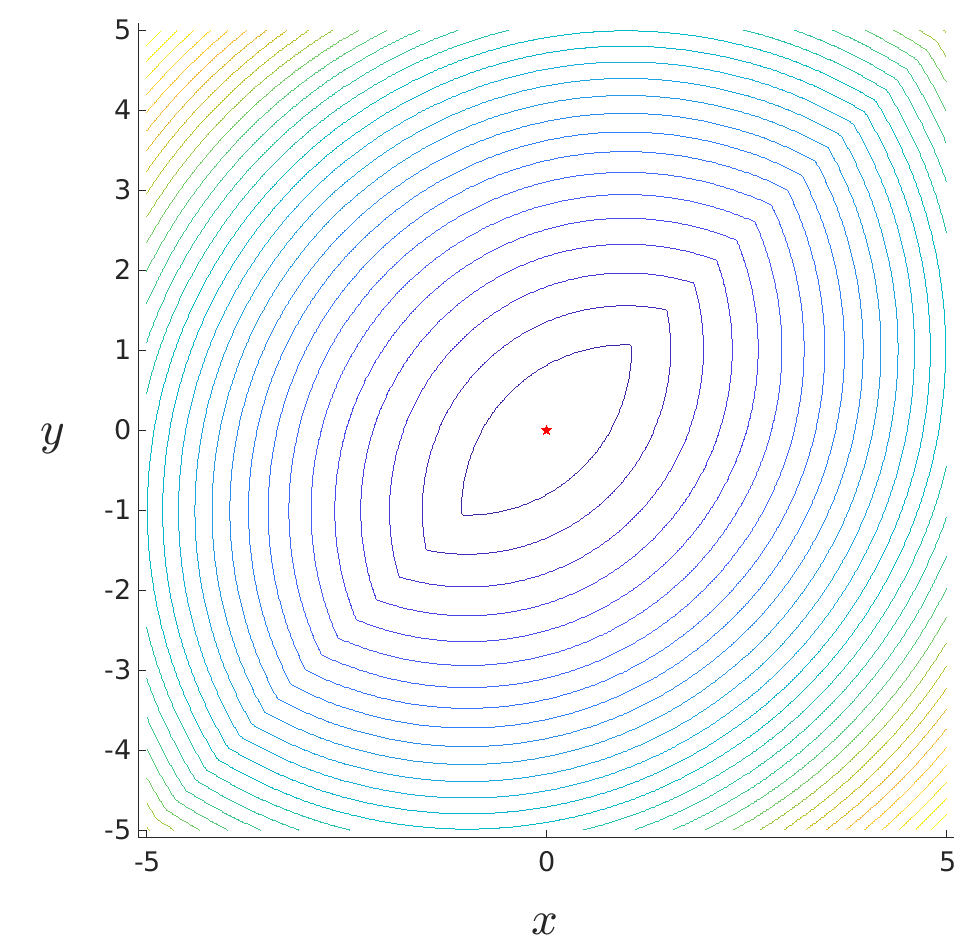
\includegraphics[scale=0.3]{./dWoods.png}
	\caption{Contours of the variant of the Dennis-Woods 
	function \eqref{eqn:dwfun}}
\label{fig:dwfun}
\end{figure}
This objective function has
a unique minimizer of $(0,0)$, and $f(0,0)=1$, indicated by a red
star in the contour plot of Fig.\,\ref{fig:dwfun}. 
The function is continuous and strictly convex everywhere,
but its gradient is discontinuous along the line $x = y$. 
It has been shown that the Nelder-Mead simplex algorithm fails to
converge to the minimizer of Dennis-Woods function\,\eqref{eqn:dwfun} in
Ref.\,\cite{dennis1987optimization}. In this subsection, we will
investigate the performance of our proposed method.

Firstly, we still examine the efficiency of the stick hill-climbing algorithm
for seeking for the neighbourhood of the minimizer $(0,0)$ of the Dennis-Woods function.
Twenty numerical experiments are performed with random 
initial values generated in the space $(-5,5)^2$. The search
radius is always fixed as $\rho=0.5$ for the set of tests. 
The stick hill-climbing algorithm can find a neighbourhood of the
minimizer $(0,0)$ in each test no matter which initial value is used.
\begin{figure}[!htbp]
	\centering
	\includegraphics[scale=0.3]{./dwoodrandInit.png}
	  \caption{The iterations of convergence of the stick
	  hill-climbing method to the Dennis-Woods function
	  \eqref{eqn:dwfun} in 20 test examples.
	  Start points are randomly generated in the space
	  $(-5, 5)^2$, and $\rho=0.5$.
	  The flat dashed line shows the average.} 
	  \label{fig:dwfun:randInit}
\end{figure}
The required iterations for convergence is shown in 
Fig.\,\ref{fig:dwfun:randInit}, while the average iterations is
about $13.5$. In these cases, the stick hill-climbing method
demonstrates a pronounced convergent behavior, even within $2$
steps.

Subsequently, we will take an example to show the numerical
behavior of the stick hill-climbing algorithm in detail. The
initial value is $(x_0, y_0)=(1.0, 1.5)$, and the search radius
is $\rho=0.5$. Tab.\,\ref{tab:dw:CHC} gives the iterative procedure.
\begin{table}[!htbp] \caption{\label{tab:dw:CHC}The convergent
	results of the stick hill-climbing algorithm with $\rho=0.5$
	when the initial value is $(x_0, y_0)=(1.0, 1.5)$. $(x^*,
	y^*)=(0,0)$, $f(x^*,y^*)=0$.}
\begin{center}
	\footnotesize{
\begin{tabular}{|c|c|c|}
 \hline
$k$ & $(x_k,y_k)$ & $|f(x_k,y_k)-f(x^*,y^*)|$ 
 \\ \hline
0 & (1.0, 1.5) & 3.125
 \\ \hline
1 &	(1.0, 1.0) & 2.0
 \\ \hline
2 & (0.64645, 0.64645)  & 1.417893
 \\ \hline
3 & (0.29289, 0.29289) &  1.085786
 \\ \hline
4 & (-0.06066, -0.06066) & 1.003680
 \\ \hline
\end{tabular}
}
\end{center}
\end{table}
The stick hill-climbing method can detect the decrease
quickly, and find a neighbourhood of the minimizer in
$4$ iterations. The convergent point is $(-0.06066,-0.06066)$. 
Using the convergent point as initial value, one can also adjust
$\rho$ in the stick hill-climbing scheme to further approach the minimizer. 	

Finally we compare the performance of the stick hill-climbing algorithm with one
of the standard directional direct-search methods, the
coordinate-search (CS) method, for the Dennis-Woods function.
Before we go further, a short introduction of the CS method is necessary. 
More details about the CS method can be found, for instance, 
in a recent monograph\,\cite{conn2009introduction} or
Ref.\,\cite{kolda2003optimization}. 
The CS method makes use of the positive bases
$\mathcal{D}_{\oplus}$ which spans the $\mathbb{R}^2$ with
positive coefficients. Let $\bmx_k$ be the current iterate and
$\lambda$ the current search step length. The CS method evaluates
the function $f$ at the points in the set
\begin{align*}
	\mathcal{P}_k = \{\bmx_k + \lambda d:
	d\in\mathcal{D}_{\oplus}\},
\end{align*}
following some specified order, trying to find a point in
$\mathcal{P}_k$ that decreases the objective function value. 
When that happens, the method defines a new iterate
$\bmx_{k+1}=\bmx_{k}+\lambda d \in \mathcal{P}_k$ such that
$f(\bmx_{k+1})<f(\bmx_{k})$. In such a case, one either leaves
the parameter $\lambda$ unchanged, or increases it, or decreases it. 
Here we will change $\lambda$ during the iterative procedure.
If none of the points in
$\mathcal{P}_k$ leads to a decrease in $f$, then the parameter
$\lambda$ is reduced (here by a factor of $1/2$) and the next
iteration at the same point ($\bmx_{k+1}=\bmx_{k}$). The
algorithm is terminated when the $\lambda$ is smaller than a
given tolerance. 

Like the CS method, the stick hill-climbing algorithm
has similar algorithmic steps to update iterates and change
the search radius. Unlike the CS method, however, the stick
hill-climbing algorithm does not predetermine the search
directions, such as $\mathcal{D}_{\oplus}$ in the CS scheme. 
In $k$ iteration, the stick hill-climbing evaluates functions on the search
surface $O(\bmx_k, \rho)$, and compares them with $f(\bmx_k)$.
In practice, the search surface $O(\bmx_k, \rho)$ is
dynamically sampled as discussed in Algorithm\,\ref{alg:refined}.
From another perspective, the stick hill-climbing algorithm
provides an adaptive mechanism to adjust the search directions 
according to objective function. 

In the following numerical tests, the initial value is $(x_0, y_0)=(1.1,
0.9)$, the initial search radius is $\rho = 1.0$.
In the stick hill-climbing algorithm, the maximum sample points $N_{\rm{max}}$
of $O(\bmx_k, \rho)$ is $8$. In the CS method, the positive bases is
$\mathcal{D}_{\oplus}=\{(1,0), (0,1), (-1,0), (0,-1)\}$ of standard choice.
The control factor of adjusting search radius $\eta=0.5$ in both methods. 
\begin{figure}[!htbp]
	\centering
	  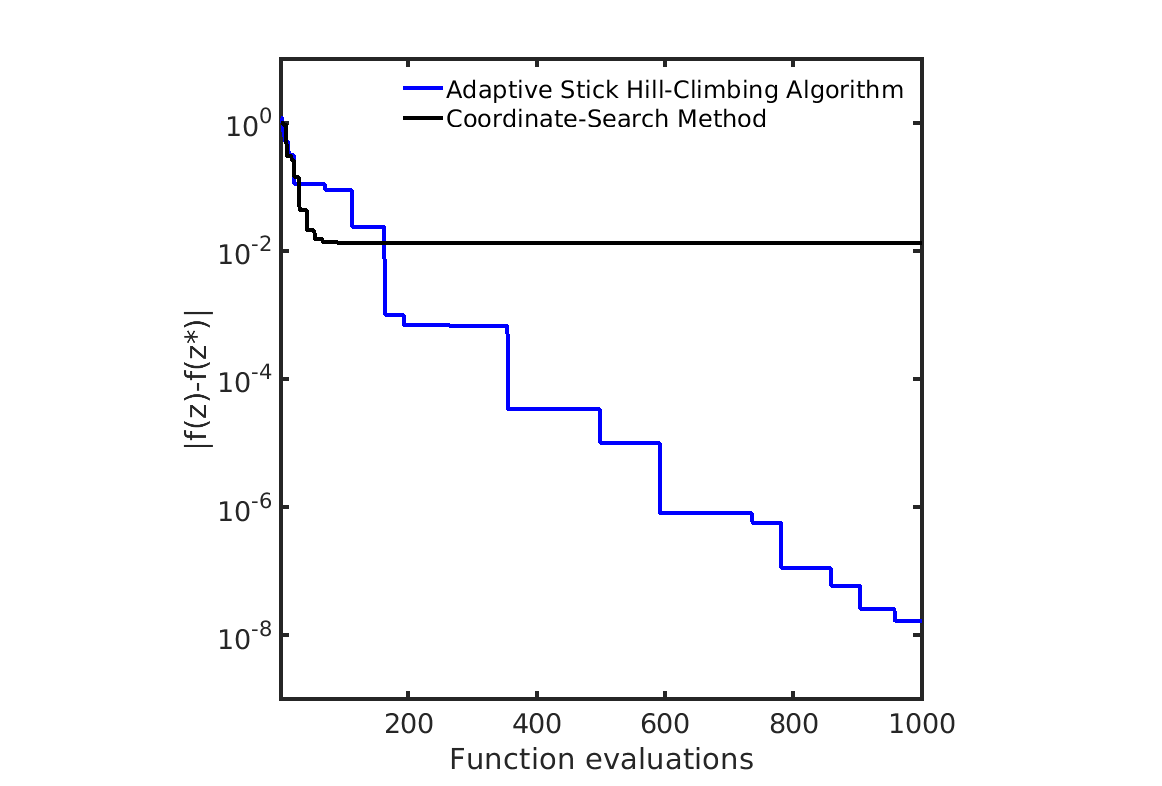
\includegraphics[scale=0.5]{./dwoods_cmp.png}
	  \caption{Application of the stick hill-climbing
	  ($N_{\max}=8$) and the CS (with predetermined search
	  directions $\mathcal{D}_\oplus$) methods to the Dennis-Woods function starting from $(x_0,
	  y_0)=(1.1, 0.9)$. In the stick hill-climbing algorithm, the
	  initial search radius $\rho = 1.0$,
	  and in the CS approach the initial search step length $\lambda=1.0$.
The control factor $\eta=0.5$ in both methods. $f(x^*,y^*)$ is
the global minimizer.}
\label{fig:dwfun:cmp}
\end{figure}

Fig.\,\ref{fig:dwfun:cmp} shows the error of
$|f(x_k,y_k)-f(x^*, y^*)|$ against the number of function
evaluations for both the stick hill-climbing and the CS method. As observed in
Fig.\,\ref{fig:dwfun:cmp} the CS method stalls at the error of 
$O(10^{-2})$, however, the stick hill-climbing method can continue to reduce
error. At an error of $2\times 10^{-9}$, the stick hill-climbing scheme 
spends $349$ function evaluations, while the iterate point is $(1.50249\times
10^{-9}, 4.48273\times 10^{-9})$, and search radius becomes
$7.45058\times 10^{-9}$.
The reason is that when the iterate approaches to the minimizer,
the CS method can not detect a sufficient decrease, even no
decrease, along the predetermined search directions in $\mathcal{D}_{\oplus}$.
This results in the stagnation phenomenon.
However, the mechanism of detecting smaller values in the stick hill-climbing algorithm 
is dependent on the feature of $f(\bmx_k)$ rather
than along predetermined directions. It yields the efficient and
flexible performance of the stick hill-climbing method when
approximating the minimizer.


\section{Conclusions and Discussion}
\label{sec:conclusion}

In this paper, we have developed a new and simple direct search
method, the stick hill-climbing algorithm, to solve unconstrained
optimization problems. 
The proposed method is inspired form the behavior of the blind for
hill-climbing with a stick to detect a higher position using circular motions.    
The main idea of the new algorithm, at each iteration, is
comparing function values on a surface of the current point,
rather than a neighbourhood of current node. 
The proposed approach has a unique parameter, the search radius
determined by the motion of the stick, which makes
the algorithm convenient in numerical implementation.
At the same time, a concrete and feasible numerical
scheme of the stick hill-climbing method, and an algorithm of tuning search radius are also presented.

Three different types of objective functions,
including single extreme point function, multi-extreme points
function, and continuous but undifferentiable function, 
were designed to test the performance of the stick hill-climbing algorithms.
So far, there is no theoretical result about the convergence and
the speed of convergence for the stick hill-climbing algorithm. 
However, numerical results demonstrate that the stick hill-climbing algorithm is
a robust scheme, and can be applied to find the neighbourhood of
extreme points when objective functions are continuous.
Furthermore, the algorithm has the following advantages. 
For an appropriate search radius, the stick hill-climbing approach can
converge in finite iterations which depends only on the search
radius rather than the initial values.
It also has potential to overcome oscillations, and find the global
minimizer, even for high-dimensional problems, by using
an appropriate search radius $\rho$, as
Sec.\,\ref{subsec:minmulit} presented. 
For an objective function with multi-extreme points, 
the proposed algorithm possesses multi-resolution
feature to distinguish the local and global optimum points  
with different values of $\rho$.
The convergent result of the stick hill-climbing method shrinks the search space and
provides a good initial value for further approximating the
extreme point. The distance between the stationary point and
convergent point is less than the search radius $\rho$. 
Therefore the stick hill-climbing scheme provides a good initial guess when
integrating with other optimization methods.
In the stick hill-climbing algorithm, the search radius plays the key role  instead of search direction.
It can approximate a maximum or a minimum to high
accuracy by itself through tuning $\rho$ during iterative procedure. 
Based on these good features, it is believed that the stick
hill-climbing algorithm has potential applications in computational science.
Meanwhile, the stick hill-climbing algorithm can be easily applied
to higher-dimensional problems and constrained optimization.

This work can be extended in several directions. The rigorous
mathematical theory should be built up, such as the convergence.
The algorithm can be applied to more higher-dimensional problems
using some well-designed techniques. Finally, applying the stick
hill-climbing algorithm to scientific problems is also
important.


\section*{Acknowledgements}
This work was supported by National Science Foundation of China 
(91430213, 11401504).
K.~Jiang was partially supported by the research grand from Hunan Science Foundation of China (2015JJ3127).


%    Insert the bibliography data here.
\begin{thebibliography}{99}

\bibitem{sun2006optimization}
W.~Y.~Sun and Y.~Yuan,
Optimization theory and methods: nonlinear programming,
New York: Springer, 2006.

\bibitem{conn2000trust}
A.~R.~Conn, N.~I.~M.~Gould and P.~L.~Toint,
Trust region methods, Philadelphia: SIAM, 2000.

\bibitem{nocedal2006numerical}
J.~Nocedal and S.~J.~Wright,
Numerical optimization, 
Berlin: Springer-Verlag, 2nd ed., 2006.

\bibitem{conn2009introduction}
A.~R.~Conn, K.~Scheinberg and L.~N.~Vicente,
Introduction to derivative-free optimization,
Philadelphia: SIAM, 2009.

\bibitem{rios2013derivative}
L.~M.~Rios and N.~V.~Sahinidis,
Derivative-free optimization: a review of algorithms and comparison
  of software implementations.
{J. Global Optim.}, 2013, 56: 1247--1293.

\bibitem{powell2000uobyqa}
M.~J.~D.~Powell, UOBYQA: unconstrained optimization by quadratic
approximation, Technical Report DAMTP NA2000/14, CMS, University
of Cambridge, 2000.

\bibitem{powell2002trust}
M.~J.~D.~Powell, On trust region methods for unconstrained
minimization without derivatives, Technical Report DAMTP
NA2002/NA02, CMS, University of Cambridge, February 2002.

\bibitem{wu2009heuristic}
T.~Wu, Y.~Yang, L.~Sun, and H.~Shao, A heuristic
iterated-subspace minimization method with pattern search for
unconstrained optimization, 
Comput. Math. Appl., 2009, 58: 2051-2059.

\bibitem{zhang2014sobolev}
Z.~Zhang, Sobolev seminorm of quadratic functions with
applications to derivative-free optimization, Math. Program.,
2014, 146: 77-96.

\bibitem{michalewicz2004how}
Z. Michalewicz and D. B. Fogel, How to solve it: modern
heuristics, Springer, 2004.

\bibitem{lecun2015deep}
Y.~LeCun, Bengio, Y.~Hinton, G.~Hinton, Deep learning, Nature,
2015, 521: 521-436.

\bibitem{hooke1961direct}
R.~Hooke and T.~A.~Jeeves,
``Direct search'' solution of numerical and statistical problems,
{J. ACM}, 1961, 8: 212--229.

\bibitem{lewis2000direct}
R.~M.~Lewis, V.~Torczon and M.~W.~Trosset,
Direct search methods: then and now,
{J. Comput. Appl. Math.},
2000, 124: 191--207.

\bibitem{nelder1965simplex}
J.~A.~Nelder and R.~Mead,
A simplex method for function minimization,
{Comput. J.}, 1965, 7: 308--313.

\bibitem{torczon1997convergence}
V.~Torczon,
On the convergence of pattern search algorithms,
{SIAM J. Optim.}, 1997, 7: 1--25.

\bibitem{kolda2003optimization}
T.~G.~Kolda, R.~W.~Lewis and V.~Torczon,
Optimization by direct search: new perspectives on some classical
and modern methods,
{SIAM Rev.}, 2003, 45: 385--482.

\bibitem{dennis1991direct}
J.~E.~Jr Dennis and V.~Torczon,
Direct search methods on parallel machines,
{SIAM J. Optim.}, 1991, 1: 448--474.

\bibitem{dieterich2012empirical}
J.~M.~Dieterich and B.~Hartke, 
Empirical review of standard benchmark functions using evolutionary global optimization,
{Appl. Math.} 2012, 3: 1552--1564.

\bibitem{gratton2015direct} 
S.~Gratton, C.~W.~Royer, L.~N.~Vicente, Z.~Zhang, Direct search
based on probabilistic descent, SIAM J.~Optim., 
2015, 25:1515-1541.

\bibitem{russell2010artificial} 
S.~J.~Russell and P.~Norvig,  Artificial intelligence: a modern
approach, 3rd ed., Prentice Hall, 2010.

\bibitem{back1996evolutionary}
T.~B{\"a}ck, 
Evolutionary algorithms in theory and practice: evolution
  strategies, evolutionary programming, genetic algorithms,
Oxford University Press, 1996.

\bibitem{dennis1987optimization}
J.~E.~Jr Dennis and D.~J.~Woods,
Optimization on microcomputers: The Nelder-Mead simplex algorithm.
In: New computing environments: microcomputers in large-scale
computing, A.~Wouk ed., Philadelphia: SIAM, 1987.

\end{thebibliography}



\end{document}
